\documentclass[final]{beamer}
\usepackage[orientation=portrait, size=a1, scale=1.4]{beamerposter}
\usepackage[spanish, es-tabla]{babel}
\usepackage[utf8]{inputenc}
\usepackage[T1]{fontenc}
\usepackage{qrcode}

%% Librerías y paquetes %%
% Paquetes matemáticos
\usepackage{amsmath, amssymb, physics, bigints, cancel}
\usepackage{stmaryrd}

% Colores y cuadros
\usepackage[table, xcdraw, x11names]{xcolor}
\usepackage[most]{tcolorbox}
\usepackage[absolute,overlay]{textpos}
\usefonttheme[onlymath]{serif}

\definecolor{ForestGreen}{rgb}{0.13, 0.55, 0.13}
\definecolor{esmerald}{RGB}{80, 200, 120}
\definecolor{gold}{RGB}{212, 175, 55}
\definecolor{silver}{RGB}{192, 192, 192}
\definecolor{lightorange}{RGB}{255, 147, 0}
\definecolor{darkorange}{HTML}{D46137}
\definecolor{lightblue}{HTML}{37AAD4}

\setlength{\TPHorizModule}{1cm}
\setlength{\TPVertModule}{1cm}

\newtcolorbox{infobox}[2][blue]{
    colback=#1!5!white,
    colframe=#1!75!black,
    title={#2},
    fonttitle=\bfseries,
    coltitle=black,
    boxrule=0.8pt,
    arc=4pt,
    left=6pt,
    right=6pt,
    top=6pt,
    bottom=6pt,
    breakable
}

% TikZ para diagramas y circuitos
\usepackage{tikz}
\usetikzlibrary{patterns, decorations.pathreplacing}
\usepackage{circuitikz}

% Figuras
\usepackage{graphicx}
\usepackage{float} % no siempre necesario, pero puede ayudar
\usepackage{booktabs}

% Formatos 
\usepackage{fontawesome}
\newcommand{\colorcancel}[2]{\textcolor{#1}{\cancel{\textcolor{black}{#2}}}}
\usepackage{bbold}
\newcommand*\circled[1]{\tikz[baseline=(char.base)]{
  \node[shape=circle,draw,inner sep=1.5pt] (char) {#1};}}

% Definir colores y estilo para el póster
\setbeamertemplate{background canvas}[vertical shading][bottom=white,top=white]
\setbeamercolor{structure}{fg=black}
\setbeamercolor{block title}{bg=black,fg=white}
\setbeamercolor{block body}{bg=white}

\begin{document}

% Título y autores
\begin{frame}[t]{}

    \begin{center}
    
        \Huge{Producción de ondas gravitacionales en el universo temprano}
    
        \vspace{0.25cm}
        
        \Large{Tomás A. Ciccarella\textsuperscript{1}, Nahuel Mirón Granese\textsuperscript{1,2,3}}

        \vspace{0.5cm}

        \small{\textit{\textsuperscript{1}Universidad de Buenos Aires (UBA), Facultad de Ciencias Exactas y Naturales (FCEN), Departamento de Física; \textsuperscript{2}Consejo Nacional de Investigaciones Científicas y Técnicas (CONICET), \textsuperscript{3}Universidad Nacional de La Plata, Facultad de Ciencias Astronómicas y Geofísicas}}
    \end{center}

    \begin{textblock*}{5cm}(3cm,1cm) 
        
\includegraphics[scale=0.7]{logo_df.png}
    \end{textblock*}
    \begin{textblock*}{5cm}(52cm,0.75cm)
        
\includegraphics[scale=0.55]{logo_uba.png}
    \end{textblock*}

    \vspace{-1.5cm}

    % Introducción teórica
    \begin{columns}[t]
        \begin{column}{0.7\textwidth}
            \begin{infobox}[cyan]{\centering ¿Qué son las Ondas Gravitacionales?}
                \begin{columns}
                    \begin{column}{0.6\linewidth}
                        \begin{itemize}
                            \item[\textcolor{brown}{$\bullet$}] Las ondas gravitacionales (GW) son perturbaciones tensoriales del espacio-tiempo que se propagan a la velocidad de la luz.
                            
                            \vspace{-1cm}

                            \begin{equation*}
                                g_{\mu \nu} = \bar{g}_{\mu \nu} + h_{\mu \nu}, \quad |h_{\mu \nu}| \ll |\bar{g}_{\mu \nu}|
                            \end{equation*}

                            \item[\textcolor{brown}{$\bullet$}] Tienen dos polarizaciones independientes, $h_{+}$ y $h_{\times}$.
                            
                            \item[\textcolor{brown}{$\bullet$}] La dinámica de estas ondas está dada por 
                            
                            \vspace{-0.5cm}

                            \begin{equation*}
                                \ddot{h}_{ij}^{TT} + 3H\dot{h}_{ij}^{TT} - \frac{1}{a^2}\nabla^2 h_{ij}^{TT} = \frac{16\pi G}{a^2}\Pi_{ij}^{TT}
                            \end{equation*}
                        \end{itemize}
                    \end{column} \hspace{-3cm}
                    \begin{column}{0.3\linewidth}
                        \begin{figure}[H]
                            \begin{tikzpicture}
                                \draw (0,0) circle (0.5cm);
                                \draw (5,0) circle (0.5cm);
                                \draw (5,-5) circle (0.5cm);
                                \draw (0,-5) circle (0.5cm);
                                \draw (2.5,0) circle (0.5cm);
                                \draw (2.5,-5) circle (0.5cm);
                                \draw (0,-2.5) circle (0.5cm);
                                \draw (5,-2.5) circle (0.5cm);

                                \draw[-{Latex}, thick, color = red] (0,0) -- (-1,1);
                                \draw[-{Latex}, thick, color = red] (0,0) -- (1,-1);
                                \draw[-{Latex}, thick, color = red] (5,-5) -- ++(-1,1);
                                \draw[-{Latex}, thick, color = red] (5,-5) -- ++(1,-1);
                                \draw[-{Latex}, thick, color = red] (5,0) -- ++(1,1);
                                \draw[-{Latex}, thick, color = red] (5,0) -- ++(-1,-1);
                                \draw[-{Latex}, thick, color = red] (0,-5) -- ++(1,1);
                                \draw[-{Latex}, thick, color = red] (0,-5) -- ++(-1,-1);

                                \draw[-{Latex}, thick, color = ForestGreen] (2.5,0) -- ++(0,1.5);
                                \draw[-{Latex}, thick, color = ForestGreen] (2.5,0) -- ++(0,-1.5);
                                \draw[-{Latex}, thick, color = ForestGreen] (2.5,-5) -- ++(0,1.5);
                                \draw[-{Latex}, thick, color = ForestGreen] (2.5,-5) -- ++(0,-1.5);
                                \draw[-{Latex}, thick, color = ForestGreen] (0,-2.5) -- ++(1.5,0);
                                \draw[-{Latex}, thick, color = ForestGreen] (0,-2.5) -- ++(-1.5,0);
                                \draw[-{Latex}, thick, color = ForestGreen] (5,-2.5) -- ++(1.5,0);
                                \draw[-{Latex}, thick, color = ForestGreen] (5,-2.5) -- ++(-1.5,0);

                                \draw (8,0) rectangle (10,-2);
                                \node at (9,-0.5) {\textcolor{red}{$h_{\times}$}};
                                \node at (9,-1.5) {\textcolor{ForestGreen}{$h_{+}$}};
                            \end{tikzpicture}
                        \end{figure}
                    \end{column}
                \end{columns}
            \end{infobox}
        \end{column}
        \begin{column}{0.3\textwidth}
            \vspace{0.75cm}
            \begin{figure}[H]
                \centering
                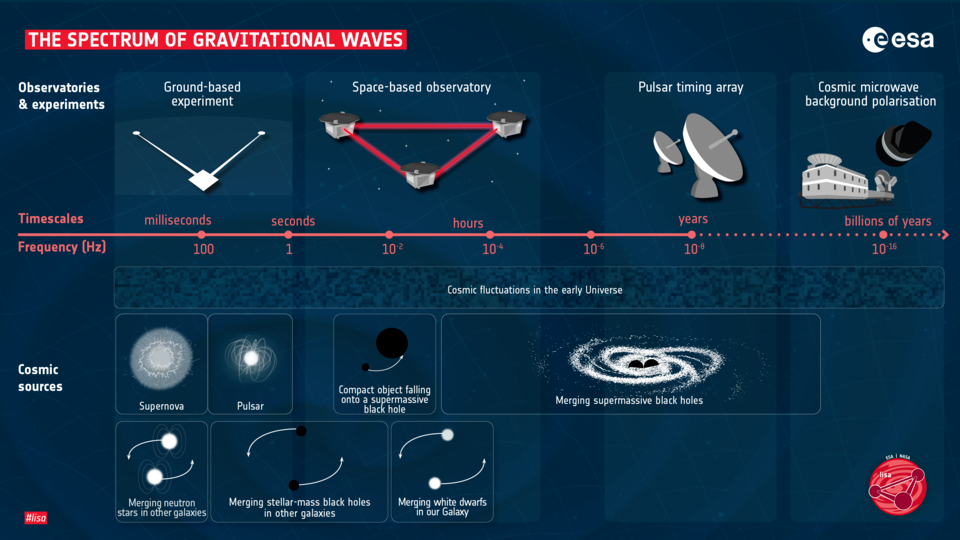
\includegraphics[width = \linewidth]{GW_fuentes.png}
            \end{figure}
        \end{column}
    \end{columns}

    \vspace{-0.5cm}

    % Explicación de reheating y producción de GW
    \begin{columns}[t]
        \begin{column}{0.5\textwidth}
            \begin{infobox}[lightorange]{\centering Reheating}
                \begin{columns}
                    \begin{column}{0.5\linewidth}
                        \begin{itemize}
                            \item[\textcolor{brown}{$\bullet$}] Luego de inflación, el universo tiene un período de transición hacia una época de radiación, conocido como \textit{reheating}.
                            
                            \item[\textcolor{brown}{$\bullet$}] Se utiliza como condición inicial para reheating la ruptura del \textit{slow-roll} inflacionario.  
                        \end{itemize}
                    \end{column}
                    \begin{column}{0.5\linewidth}
                        \begin{itemize}
                            \item[\textcolor{brown}{$\bullet$}] Durante este período, el inflatón oscila alrededor del mínimo del potencial, transfiriendo su energía a otras partículas.
                            
                            \item[\textcolor{brown}{$\bullet$}] Este proceso puede ser de forma perturbativa o no perturbativa, siendo este último conocido como \textit{preheating}.
                        \end{itemize}
                    \end{column}
                \end{columns}
                \begin{figure}[H]
                    \centering
                    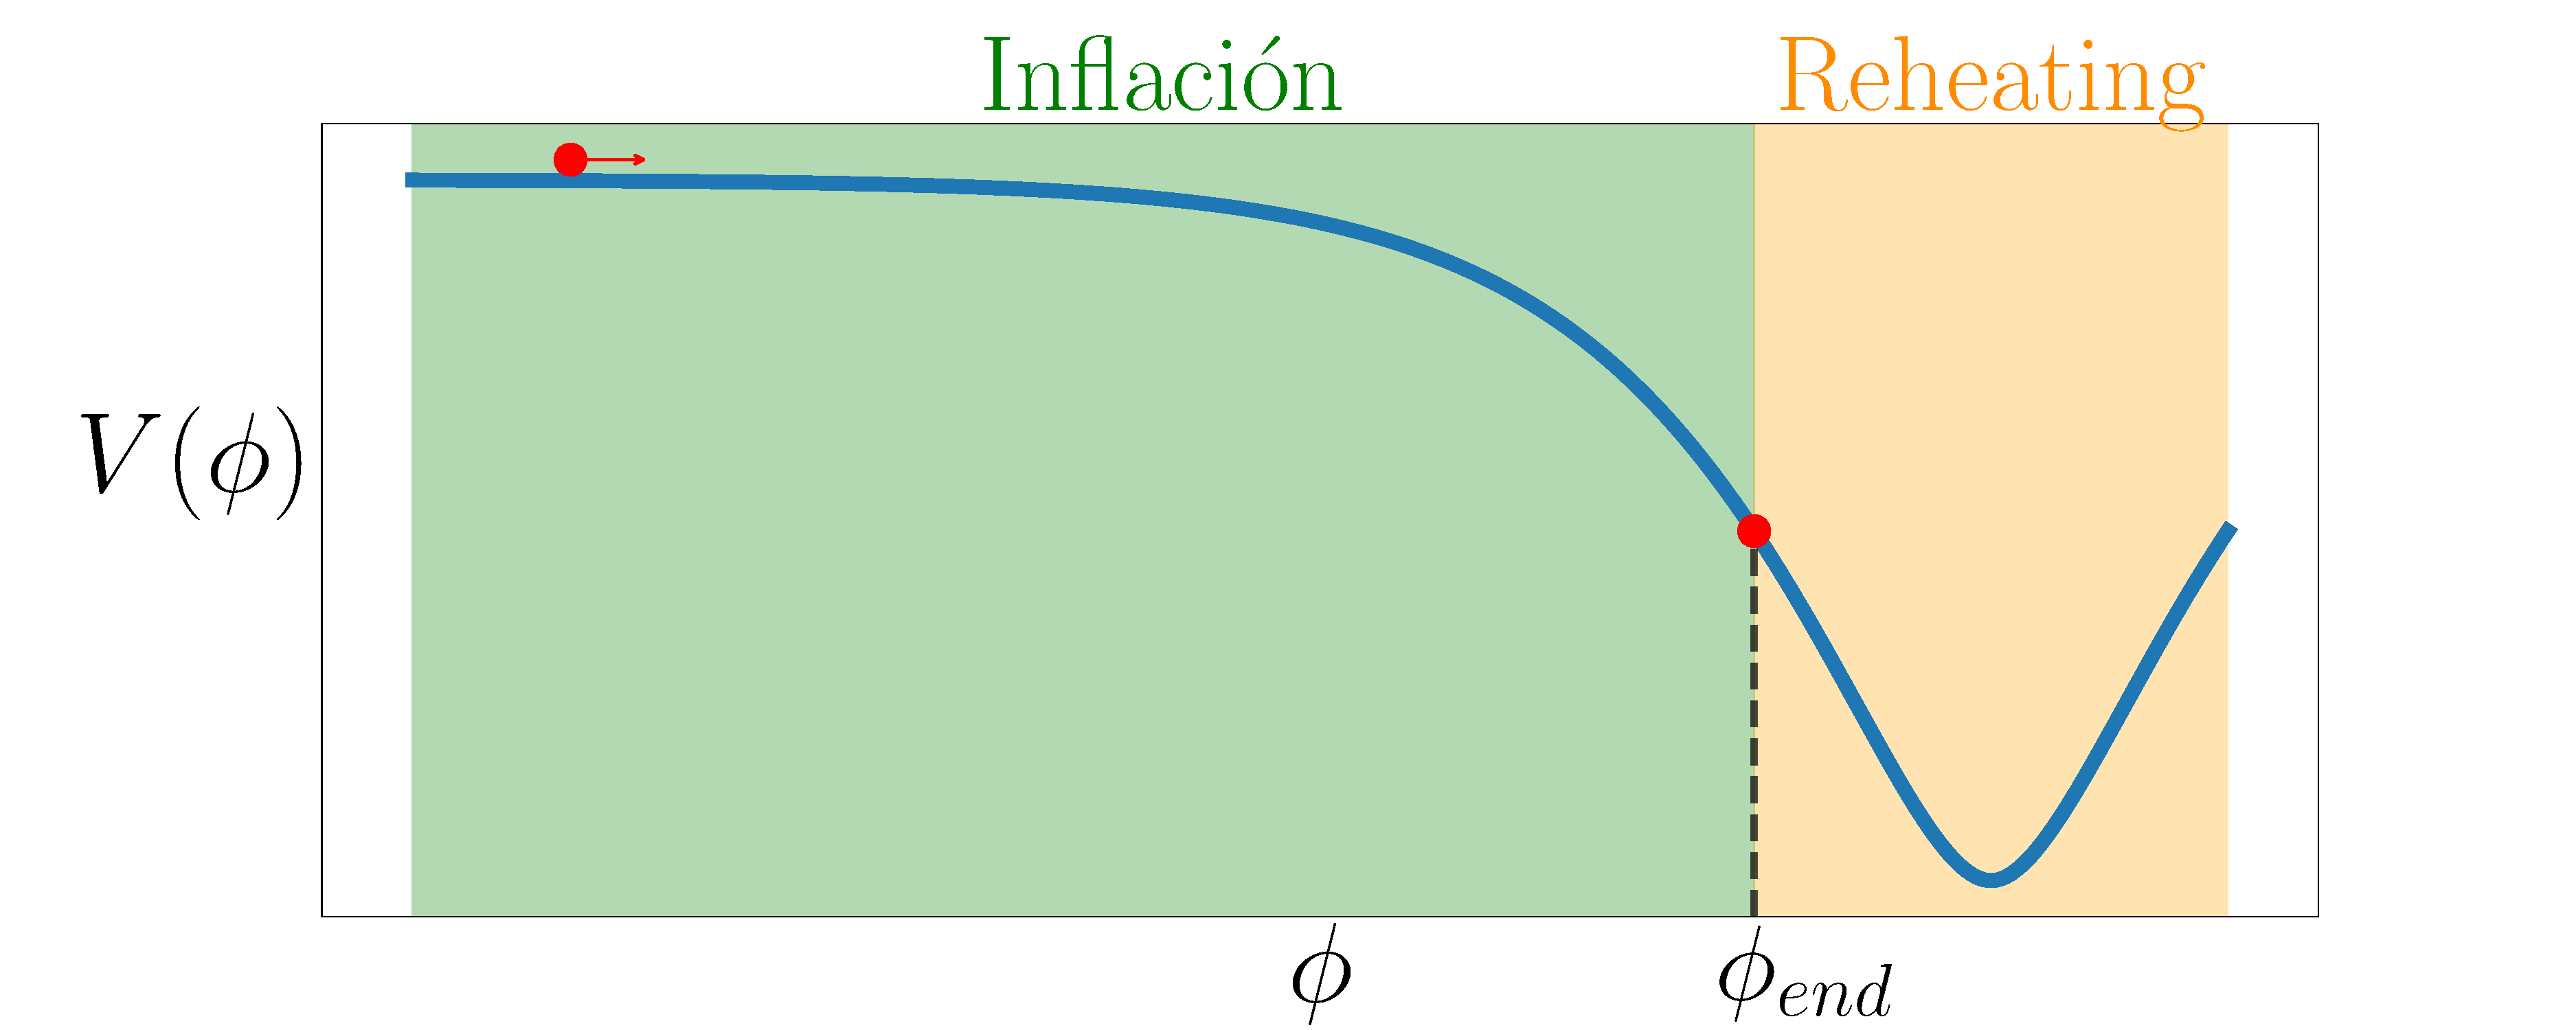
\includegraphics[width = 0.8\linewidth]{reheating}
                \end{figure}
            \end{infobox}
        \end{column}
        \begin{column}{0.5\textwidth}
            \begin{infobox}[green]{\centering Producción de GW en el universo temprano}
                \begin{itemize}
                    \item[\textcolor{brown}{$\bullet$}] Algunos mecanismos de producción de GW son:
                    \begin{itemize}
                        \item[\textcolor{blue}{$\centerdot$}] Fluctuaciones cuánticas durante inflación.
                        \item[\textcolor{blue}{$\centerdot$}] Transiciones de fase.
                        \item[\textcolor{blue}{$\centerdot$}] Dinámica de campos de materia.
                    \end{itemize}

                    \item[\textcolor{brown}{$\bullet$}] En este trabajo, nos enfocamos en la producción de GW durante el período de \textit{reheating} posterior a la inflación a partir de la dinámica de campos de materia.
                    
                    \vspace{-0.65cm}
                    
                    \begin{equation*}
                        \Pi^{TT}_{ij} = \left\{ \partial_i \phi \partial_j \phi + \partial_i \chi \partial_j \chi \right\}^{TT}
                    \end{equation*}

                    \begin{itemize}
                        \item[\textcolor{blue}{$\Rightarrow$}] Ésto funciona como fuente de GW. Y utilizando la ecuación de Einstein podemos estudiar la producción y evolución de las mismas.
                    \end{itemize}
                \end{itemize}

                \vspace{-0.35cm}

                \begin{figure}[H]
                    \centering
                    \begin{tikzpicture}
                        \filldraw[color = esmerald, opacity = 0.5] (0,-3.25) rectangle (4,3.25);
                        \filldraw[color = orange, opacity = 0.3] (4,-3.25) rectangle (16,3.25);
                        \filldraw[color = violet, opacity = 0.3] (16,-3.25) rectangle (20,3.25);
                        \draw[-{Latex}] (-1,0) -- (21,0) node[right] {$t$};

                        \draw[-{Latex}, very thick] (4,3.75) -- (0,3.75);
                        \node at (2,4.25) {Inflación};
                        \draw[decorate,decoration={brace,amplitude=10pt}] (4,3.55) -- (16,3.55) node[midway,above=10pt]{Reheating};
                        \draw[-{Latex}, very thick] (16,3.75) -- (20,3.75);
                        \node at (18,4.25) {Radiación};

                        \draw[-{Latex}] (4.5,-2.5) -- (4.5,0);
                        \draw (4.5,-2.5) -- (5,-2.5) node[right] {\shortstack{\small{Producción de partículas}\\ \small{(\textit{preheating})}}};
                        \draw[-{Latex}, color = blue, very thick] (6.5,2.5) -- (6.5,0);
                        \draw[color = blue, very thick] (6.5,2.5) -- (7,2.5) node[right, color = black] {\textbf{\small{Producción de GW}}};
                        \draw[-{Latex}] (9.5,-1) -- (9.5,0);
                        \draw (9.5,-1) -- (10,-1) node[right] {\shortstack{\small{Turbulencia}\\ \small{(efectos no lineales)}}};
                        \draw[-{Latex}] (15.5,1) -- (15.5,0);
                        \draw (15.5,1) -- (15,1) node[left] {\small{Termalización}};

                        \draw[-{Latex}] (17.5,1) -- (17.5,0);
                        \draw (17.5,1) -- (18,1) node[right] {\small{BBN}};
                    \end{tikzpicture}
                \end{figure}
            \end{infobox}
        \end{column}
    \end{columns}

    % Mathieu
    \begin{infobox}[esmerald]{\centering Evolución lineal de los campos en preheating}
        \begin{columns}
            \begin{column}{0.32\linewidth}
                \begin{infobox}[gold]{Tabla de inestabilidades de Mathieu}
                    \begin{figure}[H]
                        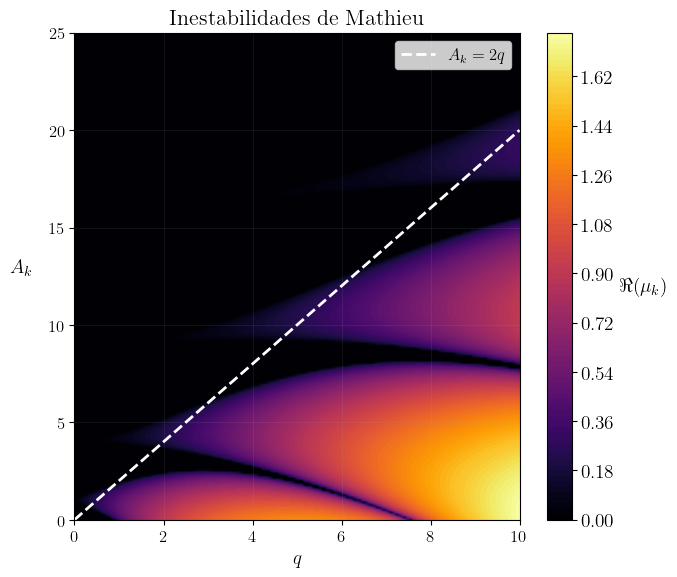
\includegraphics[width = 0.95\linewidth]{Mathieu_tabla.png}
                    \end{figure}

                    \begin{itemize}
                        \item[\textcolor{brown}{$\bullet$}] La ecuación de Mathieu da una resonancia paramétrica que sirve para ver cómo evoluciona un campo hijo $\chi$ acoplado a un campo inflatón $\phi$.
                        
                        \begin{equation*}
                            \frac{d^2 \chi_k}{dT^2} + \left[ A_k - 2q \cos(2T) \right] \chi_k = 0
                        \end{equation*}

                        \item[\textcolor{brown}{$\bullet$}] Dependiendo de los parámetros $A_k$ y $q$, se pueden encontrar regiones de estabilidad e inestabilidad. Y eso se puede leer en la tabla de inestabilidades.
                    \end{itemize}
                \end{infobox}
            \end{column}
            \begin{column}{0.32\linewidth}
                \begin{infobox}[lightblue]{Tipos de resonancia}
                    \begin{itemize}
                        \item[\textcolor{brown}{$\bullet$}] La ecuación de Mathieu tiene por solución algo de la forma $\chi_k = \mathcal{M} e^{\mu_k T}$, donde $\mu_k$ es el exponente de Floquet y $\mathcal{M}$ es una función periódica.
                    \end{itemize} 

                    \begin{figure}[H]
                        \centering
                        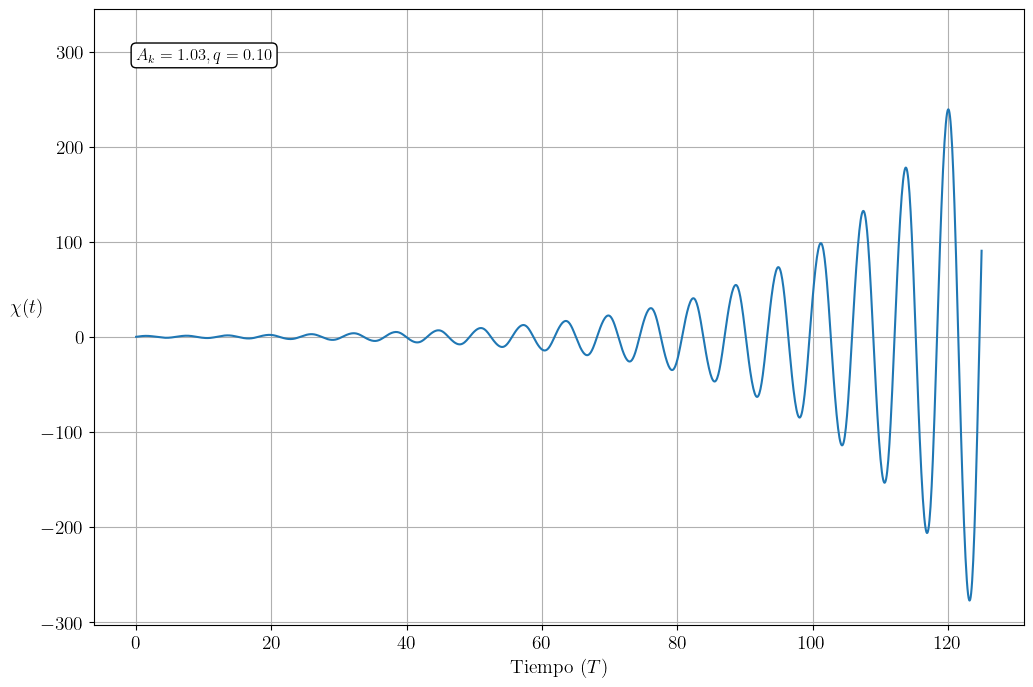
\includegraphics[width = 0.72\linewidth]{narrow_resonance.png}
                    \end{figure}

                    \vspace{-0.5cm}
                    \centering \small{Narrow resonance: $q \ll 1$. La resonancia ocurre en bandas estrechas de $k$.}

                    \vspace{1cm}

                    \begin{figure}[H]
                        \centering
                        \includegraphics[width = 0.72\linewidth]{broad_resonance.png}
                    \end{figure}

                    \vspace{-0.5cm}
                    \centering \small{Broad resonance: $q \gg 1$. La resonancia ocurre en un rango amplio de $k$.}
                \end{infobox}
            \end{column}
            \begin{column}{0.32\linewidth}
                \begin{infobox}[darkorange]{Evolución de los campos con expansión}
                    \begin{itemize}
                        \item[\textcolor{brown}{$\bullet$}] La dinámica de los campos cuando se tiene expansión del universo está regida por el siguiente sistema de ecuaciones: 
                        
                        \small{\begin{equation*}
                            \begin{cases}
                                \displaystyle \ddot{\phi} + 3 H \dot{\phi} + V_{,\phi} (\phi) = 0 \vspace{0.3cm}\\
                                \displaystyle \frac{\ddot{a}}{a} = - \frac{1}{3 m_p^2} \left[ \dot{\phi}^2 - V (\phi) \right]
                            \end{cases}
                        \end{equation*}

                        \begin{equation*}
                            \begin{cases}
                                \displaystyle \delta \ddot{\phi}_k + 3 H ~ \delta \dot{\phi}_k + \left[ \frac{k^2}{a^2} + V_{,\phi \phi} (\phi) \right] \delta \phi_k = 0 \vspace{0.3cm}\\
                                \displaystyle \ddot{\chi}_k + 3 H \dot{\chi}_k + \left( \frac{k^2}{a^2} + g^2 \phi^2 \right) \chi_k = 0
                            \end{cases}
                        \end{equation*}}
                    \end{itemize}

                    \begin{figure}[H]
                        \centering
                        \includegraphics[width = 0.88\linewidth]{Mathieu_background.png}
                    \end{figure}

                    \begin{figure}[H]
                        \centering
                        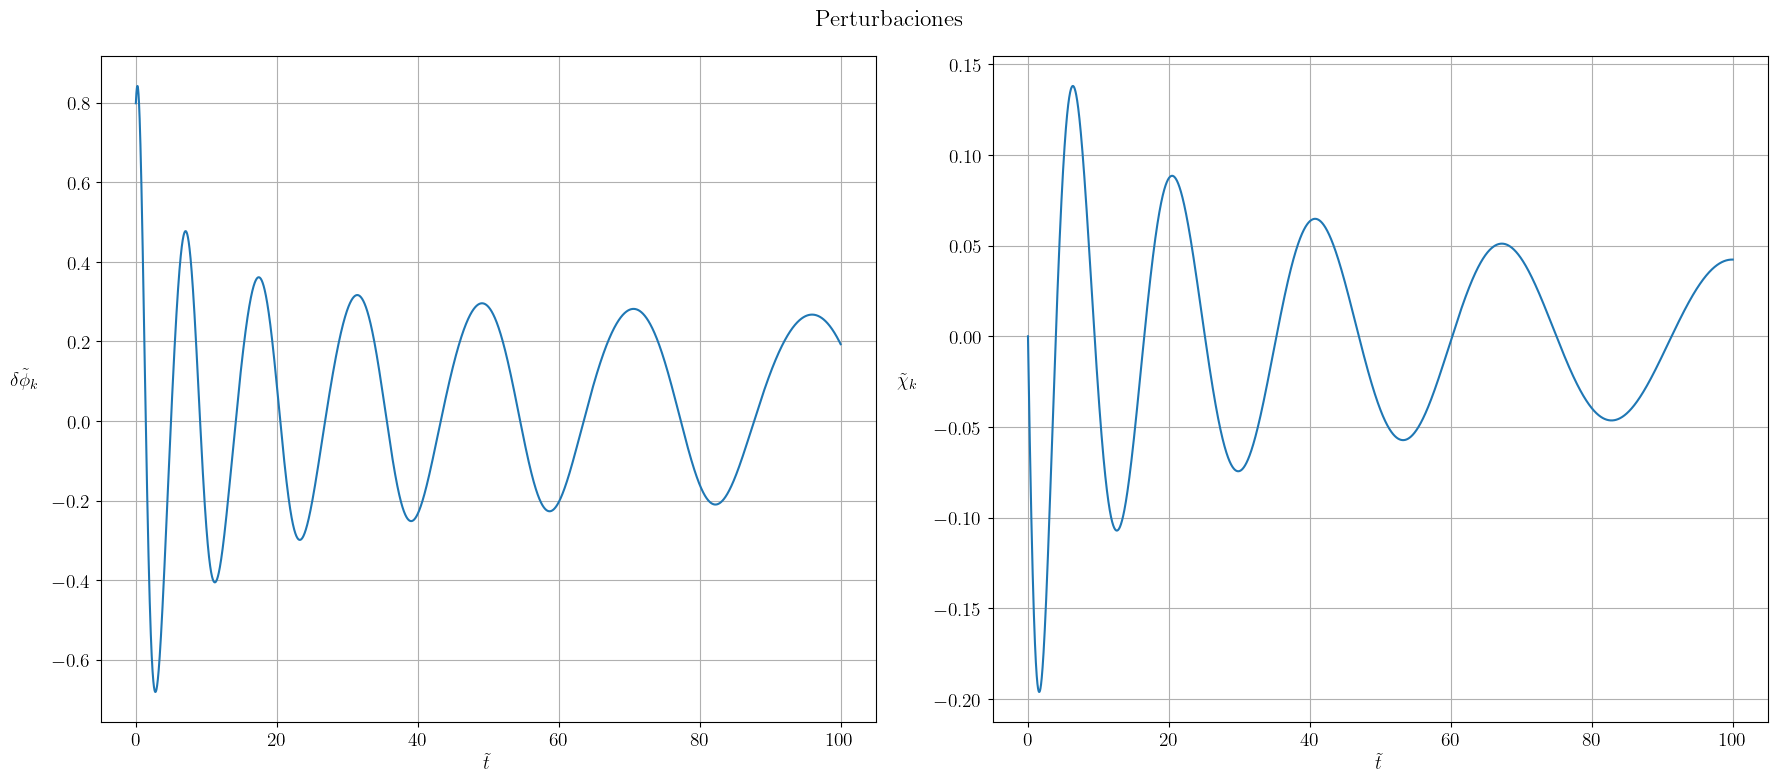
\includegraphics[width = 0.88\linewidth]{Mathieu_pert.png}
                    \end{figure}
                \end{infobox}
            \end{column}
        \end{columns}
    \end{infobox}

    \vspace{-0.5cm}

    % Cosmolattice
    \begin{infobox}[silver]{\centering Cosmolattice}
        \begin{itemize}
            \item[\textcolor{brown}{$\bullet$}] CosmoLattice es un paquete de simulaciones de tipo \textit{lattice} para simular la dinámica de campos cuando se tiene expansión del universo.
            
            \item[\textcolor{brown}{$\bullet$}] Resulta una herramienta numérica para poder trabajar con la física del universo temprano.
            
            \item[\textcolor{brown}{$\bullet$}] Se propone usar CosmoLattice para poder estudiar distintos modelos de reheating y su producción de ondas gravitacionales.
        \end{itemize}

        \begin{columns}
            \begin{column}{0.3\linewidth}
                \begin{figure}[H]
                    \centering
                    \includegraphics[width = 0.7\linewidth]{cosmolattice_1.png}
                \end{figure}

                \vspace{-0.5cm}
                \centering \small{Dinámica del campo inflatón utilizando un modelo $\lambda \phi^4$}

            \end{column}
            \begin{column}{0.3\linewidth}
                \begin{figure}[H]
                    \centering
                    \includegraphics[width = 0.7\linewidth]{cosmolattice_2.png}
                \end{figure}

                \vspace{-0.5cm}
                \centering \small{Dinámica del campo hijo utilizando un modelo $\lambda \phi^4$}
            \end{column}
            \begin{column}{0.3\linewidth}
                \begin{figure}[H]
                    \centering
                    \includegraphics[width = 0.7\linewidth]{cosmolattice_GW.png}
                \end{figure}

                \vspace{-0.5cm}
                \centering \small{Espectro de GW hoy utilizando un modelo $\lambda \phi^4$}
            \end{column}
        \end{columns}
    \end{infobox}
\end{frame}

\end{document}